\section{Contract languages}
\label{languages}

A range of languages for smart contracts exists. Figure \ref{fig:lang} gives an overview of the implementation levels of languages.
The approach in (A) is often used to allow program optimisation and verification (e.g. \cite{Lattner2004}). 
Among the projects that follow this approach are the future Ethereum development with Yul \cite{EthereumFoundation2018IULIA}, and Tezos with Liquidity \cite{OCamlProSAS2018} and Michelson \cite{DynamicLedgerSolutions2017}.
Likewise, Scilla based on Coq is intended to represent an IR that is targeted by more general languages and compiles down to be executed on a distributed VM \cite{Sergey2018}.

Smart contracts are a comparably new discipline with Bitcoin being ten years old and Ethereum a bit older than three years.
Hence, in the early stages smart contracts were designed differently as represented by (B).
Bitcoin and Bitcoin Script \cite{BitcoinWiki2018Script} skip any high-level language altogether and programmers need to write code directly in the low-level stack-based language.
Ethereum, on the other hand, offers multiple high-level languages like Solidity \cite{Ethereum2018Solidity} and Vyper \cite{Ethereum2018Vyper}.
These languages compile directly to EVM bytecode. 

\begin{figure}
\label{fig:lang}
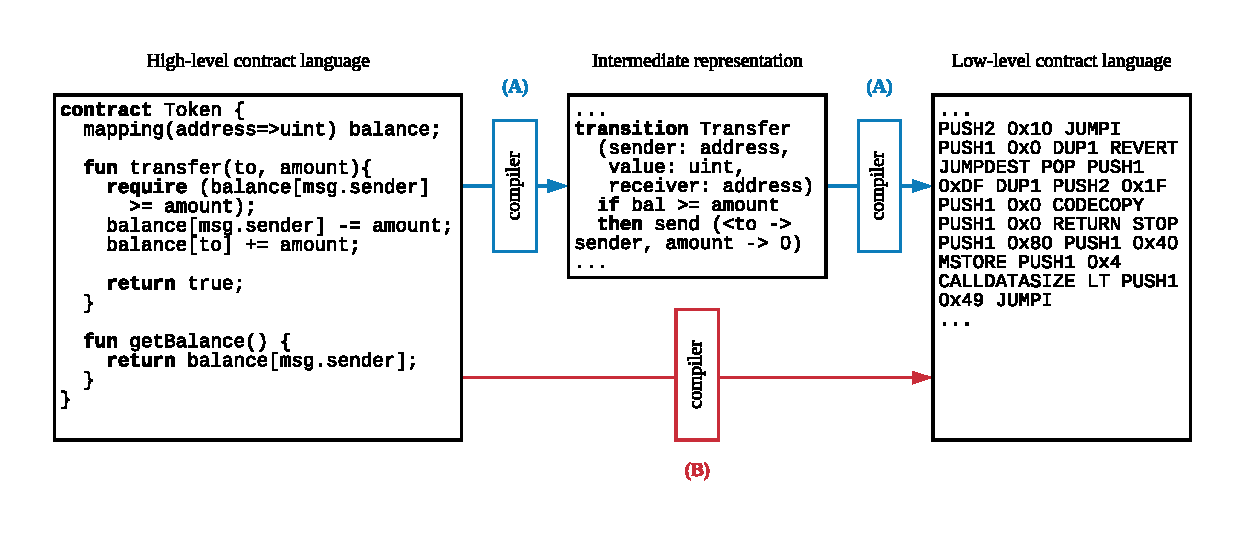
\includegraphics[width=\textwidth]{fig/Language.pdf}
\caption{Different levels of smart contract languages with syntax closely resembled to Solidity (high-level), Scilla (IR), and EVM bytecode (low-evel). (A) represents an optimised version of compiling high-level languages towards the bytecode that allows for example for verification of the IR contract and code optimisations, for example envisioned by \cite{Sergey2018,OCamlProSAS2018}. (B) represents the straightforward compilation from high-level language to bytecode representation as currently employed by Solidity and the EVM \cite{Ethereum2018Solidity,Wood2014}.}
\end{figure}


\subsection{Overview}
The overview we present in table \ref{tab:high-level} is based on five different criteria as listed below. The table gives a general overview. We explain the security properties of the languages within the following subsections.
\begin{itemize}
\item \emph{Type}: We differentiate between high-level, IR, and low-level languages.
\item \emph{Paradigm}: This describes the main paradigm of the language. Note that most languages support multiple paradigms and this criterion is more of an indication of the prevalent paradigm.
\item \emph{Instructions}: The possible instruction set that a language supports can be restricted or Turing-complete.
\item \emph{Semantics}: Languages have a formal or informal semantic. Formal semantics define the exact behaviour of programs written in that language. Informal semantics leave interpretation and mostly result in having the compiler define the exact behaviour.
\item \emph{Metering}: Smart contracts executed on a distributed ledger are re-executed by up to several thousand nodes. As these computations are costly, metering is a way to charge and limit the execution of a program.
\end{itemize}
\begin{table*}[h]
\centering
\caption{Overview of languages for smart contracts.}
\label{tab:high-level}
\begin{tabularx}{\textwidth}{XXXXXr}
\toprule
\textbf{Language} & \textbf{Paradigm} & \textbf{Instructions} & \textbf{Semantics} & \textbf{Metering} & \textbf{Ref.} \\ \toprule
\textit{Solidity} & object-oriented & Turing-complete & informal\textsuperscript{\dag} & gas, limit & \cite{Ethereum2018Solidity} \\
\textit{Vyper} & procedural & restricted & informal\textsuperscript{\dag} & gas, limit & \cite{Ethereum2018Vyper} \\
\textit{Bamboo} & procedural & Turing-complete & semi\textsuperscript{\dag} & gas, limit & \cite{Hirai2018Bamboo} \\
\textit{Flint} & procedural & Turing-complete & informal & gas, limit & \cite{Schrans2018} \\
\textit{Pyramid Scheme} & functional & Turing-complete & informal & gas, limit & \cite{Burge2018} \\
\textit{Obsidian} & object-oriented & -- & informal & -- & \cite{Coblenz2017} \\
\textit{Rholang} & concurrent & Turing-complete & informal & phlogiston & \cite{Meredith2018} \\
\textit{Liquidity} & functional & restricted & semi\textsuperscript{\dag} & gas, limit & \cite{OCamlProSAS2018} \\
\textit{DAML} & functional & restricted & -- & -- & \cite{Meier2018} \\
\textit{Pact} & functional & restricted & semi\textsuperscript{\dag} & gas, limit & \cite{Popejoy2017} \\
 \midrule
\textit{Simplicity} & pure functional & restricted & formal & -- & \cite{OConnor2017} \\
\textit{Scilla} & functional & restricted & formal & gas, limit & \cite{Sergey2018} \\
\textit{Yul} & procedural & Turing-complete & informal & gas, limit & \cite{EthereumFoundation2018IULIA} \\
%\textit{EthIR} & procedural & Turing-complete & informal & gas, limit & \cite{Albert2018} \\
\textit{IELE} & register-based & Turing-complete & formal & gas, limit & \cite{Kasampalis2018} \\ \midrule
\textit{Bitcoin Script} & stack-based & restricted & informal & script size & \cite{BitcoinWiki2018Script} \\
\textit{EVM} & stack-based & Turing-complete & informal\textsuperscript{\ddag} & gas, limit & \cite{Wood2014} \\
\textit{Bit Machine (Simplicity)} & stack-based & restricted & formal & -- & \cite{OConnor2017} \\
\textit{eWASM} & stack-based & Turing-complete & informal & gas, limit & \cite{EthereumFoundation2018ewasm} \\
\textit{Michelson} & stack-based & restricted & semi\textsuperscript{\dag} & gas, limit & \cite{DynamicLedgerSolutions2017} \\
\bottomrule
\end{tabularx}
\justify
\textsuperscript{\dag} These languages are actively developed. There are efforts to define a formal semantics. \\
\textsuperscript{\ddag} The EVM has been informally defined in \cite{Wood2014}. Formal semantics have been defined afterwards by \cite{Hirai2017,Hildenbrandt2017}.
\end{table*}


\subsection{Securing high-level languages}

A range of high-level languages exist. We noted that at this level languages try to encourage patterns that create a balance between contracts expressiveness and restrictions to encourage the secure behaviour of contract.

\paragraph{Languages:}
Solidity is the most widely used language and created for Ethereum \cite{Ethereum2018Solidity}. It resembles JavaScript, and current updates have a focus on increasing security (e.g.\ introduction of \texttt{transfer} or support for function modifiers). 
Bamboo is designed with formal verification in mind and makes state-transition explicit \cite{Hirai2018Bamboo}. 
Vyper restricts instructions (e.g.\ finite loops and no recursive calls) and prevents other features such as inheritance, function overloading, and inline assembly \cite{Ethereum2018Vyper}. 
Flint further introduces the definition of function access (by defining the address of the caller) and creates an asset type. 
Pyramid Scheme based on the Scheme is functional and imperative \cite{Burge2018}. This allows, for example, to create pure functions relatively quickly and should promote clear separation of functions that change state (i.e.\ require a transaction on the ledger being invoked) and stateless functions (i.e.\ only local calls are required).
Common to the above languages is that they target the EVM.

High-level languages are proposed for other VMs or independent from the ledger implementation.
Obsidian models contracts as finite state machines (FSM) with explicit state transition functions \cite{Coblenz2017}.
Rholang focusses on concurrency and message-passing with statically typed communication channels \cite{Meredith2018}.
Liquidity focusses on restricted instruction sets and enables formal verification by being based on OCaml \cite{OCamlProSAS2018}.
Rholang and Liquidity are intended for permissionless distributed ledgers.
DAML is functional and developed for financial applications, primarily on permissioned ledgers \cite{Shaul2018,Meier2018,Lippmeier2018,Huschenbett2018,Bernauer2018,Maric2018,Bleikertz2018,Lochbihler2018,Pilav2018}.
Similar, Pact is designed for the Kadena permissioned blockchain \cite{Popejoy2017}.
Both have a restricted instruction set and with the intention to promote formal verification.

Several other contract languages have been developed outside the context of distributed ledgers. The Business Contract Language supports creating and monitoring legal contracts \cite{Neal.2003,Governatori2006}. Specific DSLs have been created for selected use cases, for example, Quality of Service contracts \cite{Braga2009}.
Other such languages are based on a form of logic and implemented as a dialect of Prolog \cite{Michael2010}.
Further, event calculus with an XML formalisation is used model and track state of contracts \cite{Farrell2004}.
Last, it is proposed to create a language for each specific use case or user type of a contract based on a general-purpose modelling language \cite{Burge2018DSL}.

\paragraph{Paradigm:} We noted that at high-level languages support a wide range of paradigms. 
Early languages like Solidity provide a general use language that is easy to learn due to its contract-orientation similar to object-oriented programming.
Later, languages introduced functional paradigms, for example, Pyramid Scheme, Vyper, and Bamboo.
Especially languages intended for enterprise usages like Pact and DAML use functional paradigms.
Logic-based languages are interesting as they closely resemble natural language contracts and have been explored in \cite{Idelberger2016}. However, they transfer determining the implementation of statements to a lower level as ultimately, the ledger needs to be deterministic.
Additionally, languages as Rholang, Bamboo, and Obsidian as well as interfaces to Solidity \cite{Mavridou2018} make use of an FSM concept. Explicit state transitions prevent undesired or unplanned states.


\paragraph{Instructions:} The low-level language needs to be deterministic in a decentralised setting.
A range of higher languages like Vyper, Liquidity, DAML, and Pact thus restrict the language. In practice, infinite loops and recursion would block any node in the network executing the smart contract. As this is not the desired behaviour, it can be directly restricted by the language. Other languages, however, offer such constructs.
Another critical aspect of the instruction set is the possibility of calling other contracts. This can potentially introduce unexpected behaviour. Calls might terminate unexpectedly due to out-of-gas exceptions or exceptions in the called contract. 
Other restrictions might be imposed by requiring functions to be pure or restricting overriding.

\paragraph{Semantics:} Except for Bamboo, Liquidity, and Pact, semantics have been defined informally. This leaves the correct interpretation of programs to the compiler. Creating a formal semantic for a higher-level language can enable the creation of verified compilers for said language and support verification efforts.
Next, languages like Flint introduce additional types of assets. Smart contracts typically operate on some form of an asset like fungible or non-fungible tokens. Instead of using existing types, particular asset types can account for the critical handling of assets.

\paragraph{Metering:} Most languages inherit their metering mechanism from the underlying VM. DAML and Obsidian are introduced as general languages, and the use of gas is not explicitly discussed. The other languages use the concept of gas to charge computations based on resource usage and limit the overall amount of available resource by imposing a gas limit. Rholang's phlogiston essentially implements the gas concept as well.


\paragraph{Additional security properties:} 
Apart from the features that a language supports, practices can be applied to prevent the unintended behaviour.
In \cite{Wohrer2018}, present six patterns to enhance the security of Solidity smart contracts.
Further, best practice libraries are often used to prevent commonly known issues, e.g.\ \cite{ConsenSys2018Security}.
For example, integer overflows in the EVM are prevented by using explicit checks.
Moreover, templates can be used to create smart contracts \cite{Clack2016}.

\subsection{Securing intermediary languages}
IR languages aim for enabling optimisations and building a basis for verification efforts.

\paragraph{Languages:} Simplicity is a pure functional language that places itself as an intermediary representation between a higher level (functional) language and a low-level VM \cite{OConnor2017}. It compiles to a low-level language called Bit Machine. Notably, it is built in a UTXO model and is not concerned with the global state of the underlying ledger.
Scilla is functional with an automata-based design using explicit state transition functions and handling for communication patterns \cite{Sergey2018}. The semantics are defined in Coq, and formal verification is one of the primary considerations.
Yul (formerly IULIA and JULIA) is introduced as part of Solidity and its compiler \cite{EthereumFoundation2018IULIA}. The idea is to use it as an IR compilation target for multiple high-level languages and optimisations. Further, Yul aims to target the current (1.0) and planned updated EVM (1.5) as well as eWASM.
EthIR is a decompilation target for EVM bytecode \cite{Albert2018}. Its purpose is making the control and data flow of smart contracts explicit allowing analysis such as symbolic execution to operate on its code. 
IELE is derived from its formal semantics and used as an IR for smart contracts \cite{Kasampalis2018}. The syntax is similar to LLVM and has been designed using the K framework \cite{Rosu2007}.
Scilla, Yul, EthIR, and IELE use an account-based model for the blockchain with global state.

\paragraph{Paradigm:} Simplicity and Scilla use functional programming and pure functions in their language. Scilla is additionally driven by an automata-based approach with the precise definition of state transitions and terminating communications with other contracts.
EthIR presents precise data and control flow that allows building rule-based languages. This supports the security of contracts by allowing verification methods to operate on it.


\paragraph{Instructions:} Both, Simplicity and Bit Machine are not Turing complete. However, they accept finite recursions and loops. The idea is to create a language that is more expressive than Bitcoin Script but offers more security features and restrictions than the EVM. Scilla has a similar goal of restricting the instruction set. Additionally, Scilla handles global state instead of using a UTXO model.
Yul is a compilation target for Solidity and builds a layer between Solidity's high-level syntax and the bytecode of the EVM. It serves primarily as an optimisation language and hence supports native access to low-level functions.
EthIR and Yul inherit the Turing-complete instruction set of the EVM.
IELE has been developed with the intention to create a VM that enables formal verification. Although it is Turing-complete, it has differences to the EVM. Functions use registers, whose number can be statically determined. Also, arbitrary-precision signed integers are used to prevent overflows.

\paragraph{Semantics:} Simplicity and Scilla have a formal semantics defined in Coq. IELE is defined in K, and its implementation has been derived from the formal semantics. Smart contracts written in these languages can be formally verified using a specification of the contract behaviour or logic. Yul and EthIR are informally defined.

\paragraph{Metering:} For Yul and EthIR this is inherited from the EVM. However, EthIR is instead used to verify contracts than for actual execution. Therefore, the concept of gas needs to be accounted for when searching for exceptions (out.of-gas) and program analysis. Simplicity does not have explicit metering, but since it is designed for a UTXO model, one could imagine a script size restriction or a gas-based model.
Scilla and IELE use gas to charge computations and prevent over-subscription of resources.

\subsection{Securing low-level languages}
Low-level languages are the ones that represent the contract as it is executed by the nodes in the network.
They can be secured mainly by restricting their instruction set to prevent unintended behaviour and formal semantics to verify that contracts are correct.

\paragraph{Languages:}
The low-level languages in our survey are stack-based. Smart contracts are stored on a distributed ledger in the low-level language to be executed by the distributed VM.
Bitcoin scripts are a sequence of op-codes stored within one transaction in the Bitcoin network\cite{BitcoinWiki2018Script}. Hence, these contracts need to be re-written and included in the blockchain once the transaction is spent. Possible contracts are for example Hashed Timelock Contracts (HTLCs) \cite{BitcoinWiki2018HTLC}.
The EVM stores programs in the data field of an address in the Ethereum network \cite{Wood2014}. State changing functions are invoked with sending a transaction to the contract. Non-state changing functions are executed locally and do not use gas. Contract functions in the EVM have a signature that can be called by using the contract's address and its Application Binary Interface (ABI).
eWASM is a proposed successor of the EVM based on a deterministic variant of Web Assembly (WASM) \cite{Wanderer2015,EthereumFoundation2018ewasm}.
Michelson is the low-level language of the Tezos blockchain \cite{DynamicLedgerSolutions2017}. It uses accounts as well but is designed to promote formal verification.
An exception to the low-level languages stored on the blockchain is Scilla. The blockchain Zilliqa directly stores Scilla contracts on its chain.

\paragraph{Paradigm:} All languages are stack-based. Their low-level implementation makes a manual inspection of contracts cumbersome. Hence, automated tools can help to support such verification efforts. Moreover, decompilers are used to convert the stack into a higher level language.

\paragraph{Instructions:} Bitcoin script is quite restrictive. Moreover, op-codes that are defined for it are not activated in the Bitcoin blockchain due to security concerns. Nonetheless, protocols like Lightning \cite{Poon2016} can still be based on the restricted instruction set.
The EVM and eWASM, on the other hand, strive for Turing-completeness. While there is a discussion of restricting VMs for security reasons, eWASM is supposed to be backwards compatible with the EVM.
Optimisation for op-code reuse is proposed in \cite{Pontiveros2018}.
\citeauthor{Pontiveros2018} proposes to re-use EVM code to optimise the space usage of code with a new op-code. This technique could be applied to reference proven secure code patterns.
Michelson is more restrictive than EVM but less so than Bitcoin script. It seeks a balance between allowing generating expressive contracts and maintaining security properties.

\paragraph{Semantics:} Low-level languages have been informally defined. In later work, the EVM has been formally defined in K \cite{Hildenbrandt2017}, Lem \cite{Hirai2017}, and F* \cite{Grishchenko2018}. Michelson seeks to have a formal semantics before realising the main version of the language.

\paragraph{Metering:} The standard practice is to use gas and a gas limit to restrict instructions. Opposite to that, Bitcoin script uses a maximum script size of 10,000 bytes as a restriction. Merkelized Abstract Syntax Tree (MAST) is a proposal to allow larger scripts without increasing the script size limit \cite{Harding2017}.


\subsection{General purpose languages}
Apart from using DSLs for programming smart contracts, projects like Hyperledger Fabric or Neo use general purpose programming languages.
This can have advantages as those languages are already known to potential developers, and verification tools might already exist.
For example, Hyperledger Fabric uses Docker containers with smart contracts (so-called ``chaincode'') written in Go, Java, or Node.js \cite{Cachin2016}. 

However, as these languages are originally not designed for smart contracts the global state of the ledger needs to imported through special functions that are typically not available in these languages.
Moreover, these languages often have support for infinite loops and recursion which are not desirable.
Particular types like assets or units also need to be declared. 
This can be achieved by using libraries, but arguably, a developer then has to adjust to the new principles imposed by such a library.